\chapter{坐标}
一般常用的坐标系统有迪卡尔坐标、极坐标,这两种\tikzname
都提供了。可以用明确的方式指定坐标系统,也可以隐式的让\tikzname 自己推导,因为两种坐标的格式是不一样的。
\begin{texlst}
	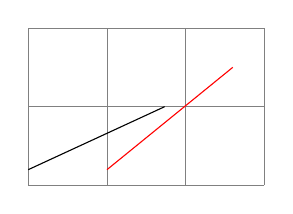
\begin{tikzpicture}
		\draw[help lines] (0,0) grid (3, 2);
		\draw(canvas cs:x=0cm, y=2mm) -- (canvas polar cs: radius=2cm, angle=30); % 显式
		\draw[red](1, 2mm) -- (30:3cm); % 隐式
	\end{tikzpicture}
\end{texlst}

坐标如果不带单位的话,默认为cm。坐标可以是$(x, y)$式的,也可以用名称,但是所有的都需要用小括号给包住。

如果需要将坐标偏移的话,需要用\texinline{([xshift=3pt] 1,1)}这种写法。

坐标支持不同单位的四则运算。
\begin{texlst}
	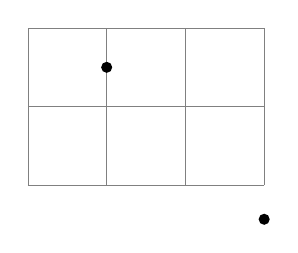
\begin{tikzpicture}
		\draw[help lines] (0,0) grid (3,2);

		\fill(canvas cs:x=1cm, y=1.5cm) circle (2pt);
		\fill(canvas cs: x=1.5 * 2cm, y=-5mm + 2pt) circle (2pt);
	\end{tikzpicture}
\end{texlst}

\section{xyz坐标系统}
\begin{texlst}
	\begin{tikzpicture}[->]
		\draw (0,0) -- (xyz cs:x=1) node[right]{$x$};
		\draw (0,0) -- (xyz cs:y=1)node[above]{$y$};
		\draw (0,0) -- (xyz cs:z=1)node[below left]{$z$};
	\end{tikzpicture}
\end{texlst}
xyz坐标系统也可以采用隐式标记的方法来书写。
\begin{texlst}
	\begin{tikzpicture}[->]
		\draw (0,0) -- (1,0);
		\draw (0,0) -- (0,1,0);
		\draw (0,0) -- (0,0,1);
	\end{tikzpicture}
\end{texlst}
此外,xyz坐标系统也支持极坐标,不过,这一块我就不考虑了。

\section{重力坐标系统barycentric}
这种坐标系统可以看到权重的偏向,一般平时也用不到。

\begin{texlst}
	\begin{tikzpicture}
		\node(c)[text width=3cm, text height=3cm, draw]{};
		\coordinate(one) at (c.north east);
		\coordinate(two) at (c.south east);
		\coordinate(three) at (c.north west);
		\coordinate(four) at (c.south west);

		\node[above=0.5cm, text width=1cm, font=\tiny, align=center] at (one){重要\\紧急};
		\node[below=0.5cm, text width=1cm, font=\tiny, align=center] at (two){紧急\\不重要};
		\node[above=0.5cm, text width=1cm, font=\tiny, align=center] at (three){重要\\不紧急};
		\node[below=0.5cm, text width=1cm, font=\tiny, align=center] at (four){不重要\\不紧急};

		\node[font=\tiny, text width=1cm] at (barycentric cs:one=1,two=0,three=0,four=0){生命受到威胁};
		\node[font=\tiny, text width=1cm] at (barycentric cs:one=0,two=1,three=0,four=0){拉肚子上厕所};
		\node[font=\tiny, text width=1cm] at (barycentric cs:one=0,two=0,three=1,four=0){保持健康};
		\node[font=\tiny, text width=1cm] at (barycentric cs:one=0,two=0,three=0.5,four=1){找朋友喝酒};
	\end{tikzpicture}
\end{texlst}
这个重力坐标图的例子没有举好,不过大概就是这么个意思。

\section{节点坐标系统}
这种坐标系统就是用节点的名字来代替实际的数字坐标。
\begin{texlst}
	\usetikzlibrary{arrows.meta}
	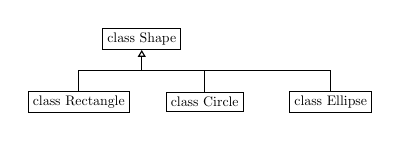
\begin{tikzpicture}[every node/.style={scale=0.5}, scale=0.4]
		\node (shape) at (0,2) [draw] {class Shape};
		\node (rect) at (-2,0) [draw] {class Rectangle};
		\node (circle) at (2,0) [draw] {class Circle};
		\node (ellipse) at (6,0) [draw] {class Ellipse};

		\draw (node cs:name=circle,anchor=north) |- (0,1);
		\draw (node cs:name=ellipse,anchor=north) |- (0,1);
		\draw [arrows=-{Triangle[open, angle=60:1mm]}] (node cs:name=rect,anchor=north) |- (0,1) -| (node
		cs:name=shape,anchor=south);
	\end{tikzpicture}
\end{texlst}
还可以使用角度来替代锚点。
\begin{texlst}
	\usetikzlibrary{shapes.geometric}
	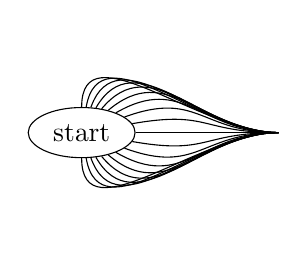
\begin{tikzpicture}
		\node (start) [draw, shape=ellipse] {start};
		\foreach \ang in {-90, -80, ..., 90}
		\draw (node cs:name=start,angle=\ang) .. controls +(\ang:1cm) and +(-1, 0) .. (2.5,0);
	\end{tikzpicture}
\end{texlst}
如果锚点和角度都没有提供的提供的话,\tikzname\ 会自动计算出一个合适的连接方式。
在实际的使用中,可以隐式的表达节点坐标系统,比如\texinline{(nodename.south)}或者\texinline{(nodename.30)}。

\section{正切坐标系统}
此坐标系统需要加载\texinline{calc}库,而且没有隐式的调用方法。
\begin{texlst}
	\usetikzlibrary{calc}
	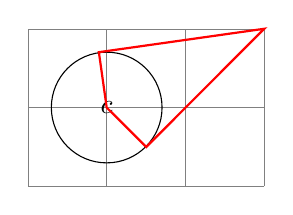
\begin{tikzpicture}
		\draw[help lines] (0,0) grid (3,2);
		\coordinate(a) at (3,2);

		\node[circle, draw] (c) at (1,1) [minimum size=40pt] {$c$};

		\draw[red, thick] (a) -- (tangent cs:node=c,point={(a)},solution=1) -- (c.center) -- (tangent
		cs:node=c,point={(a)},solution=2) -- cycle;
	\end{tikzpicture}
\end{texlst}

手册里面还提到了一种自定义坐标系统的方法,不过我没有看懂,这个也不是目前的重点,先略过。

\section{交点}
\texinline{(2,1 |- 3,4)}这种写法可以得到从\texinline{(2,1)}先垂直后水平方向得到交点。如下面图标:
\begin{texlst}
	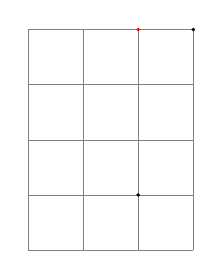
\begin{tikzpicture}[scale=0.7]
		\draw[help lines](0,0)grid(3,4);
		\fill(2,1) circle (1pt);
		\fill(3,4) circle (1pt);
		\fill[red](2,1 |- 3,4) circle (1pt);
	\end{tikzpicture}
\end{texlst}

还有一种方法是需要载入\texinline{intersections}库来实现,请先看一个简单的示例:
\begin{texlst}
	\usetikzlibrary{intersections}
	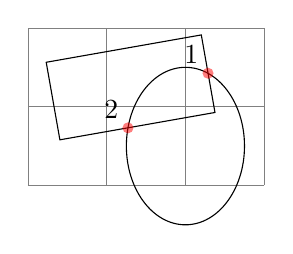
\begin{tikzpicture}[every node/.style={opacity=1, black, above left}]
		\draw [help lines] grid (3, 2);
		\draw [name path=ellipse] (2,0.5) ellipse(0.75cm and 1cm);
		\draw [name path=rectangle, rotate=10] (0.5, 0.5) rectangle +(2,1);
		\fill [red, opacity=0.5, name intersections={of=ellipse and rectangle}]
		(intersection-1) circle (2pt) node {1}
		(intersection-2) circle (2pt) node {2};
	\end{tikzpicture}
\end{texlst}

这里默认的名字就叫\texinline{intersection-数字},我们也可以自己设置交点的名称。另外还可以交点的总数设置给变量。来看下面一个例子:
\begin{texlst}
	\usetikzlibrary{intersections}
	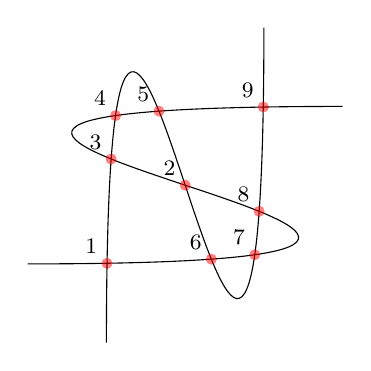
\begin{tikzpicture}
		\clip (-2, -2) rectangle (2, 2);
		\draw[name path=curve 1] (-2,-1) .. controls (8,-1) and (-8,1) .. (2,1);
		\draw[name path=curve 2] (-1,-2) .. controls (-1,8) and (1, -8) .. (1,2);
		\fill [name intersections={of=curve 1 and curve 2, name=i, total=\t}]
		[red, opacity=0.5, every node/.style={ above left, black, opacity=1 }]
		\foreach \s in {1,...,\t} {(i-\s) circle (2pt) node {\footnotesize\s}};
	\end{tikzpicture}
\end{texlst}

还可以用\texinline{by}来给交点命名。
\begin{texlst}
	\usetikzlibrary{intersections}
	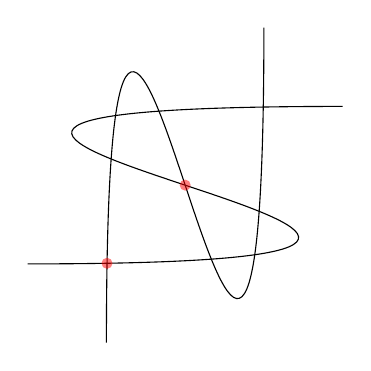
\begin{tikzpicture}
		\clip (-2, -2) rectangle (2, 2);
		\draw[name path=curve 1] (-2,-1) .. controls (8,-1) and (-8,1) .. (2,1);
		\draw[name path=curve 2] (-1,-2) .. controls (-1,8) and (1, -8) .. (1,2);
		\fill [name intersections={of=curve 1 and curve 2, by={a, b}}]
		[red, opacity=0.5, every node/.style={ above left, black, opacity=1 }]
		(a) circle (2pt)
		(b) circle (2pt);
	\end{tikzpicture}
\end{texlst}

甚至还可以用\texinline{foreach}的语法来给交点加上\texinline{lable}。
\begin{texlst}
	\usetikzlibrary{intersections}
	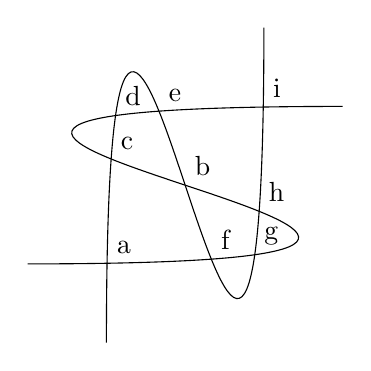
\begin{tikzpicture}
		\clip (-2, -2) rectangle (2, 2);
		\draw[name path=curve 1] (-2,-1) .. controls (8,-1) and (-8,1) .. (2,1);
		\draw[name path=curve 2] (-1,-2) .. controls (-1,8) and (1, -8) .. (1,2);
		\fill [name intersections={of=curve 1 and curve 2, by={
							[label=above right:a],[label=above right:...], [label=above right:i]}}];
	\end{tikzpicture}
\end{texlst}

用\texinline{sort by}来根据某条路径来排列交点的顺序。
\begin{texlst}
	\usetikzlibrary{intersections}
	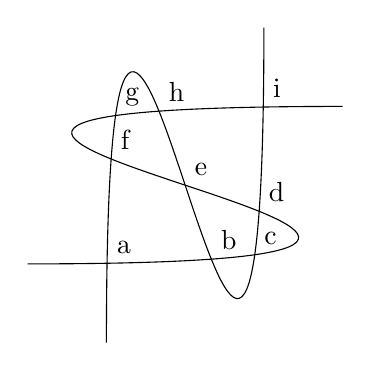
\begin{tikzpicture}
		\clip (-2, -2) rectangle (2, 2);
		\draw[name path=curve 1] (-2,-1) .. controls (8,-1) and (-8,1) .. (2,1);
		\draw[name path=curve 2] (-1,-2) .. controls (-1,8) and (1, -8) .. (1,2);
		\fill [name intersections={of=curve 1 and curve 2, sort by=curve 1, by={
							[label=above right:a],[label=above right:...], [label=above right:i]}}];
	\end{tikzpicture}
\end{texlst}

\begin{texlst}
	\usetikzlibrary{intersections}
	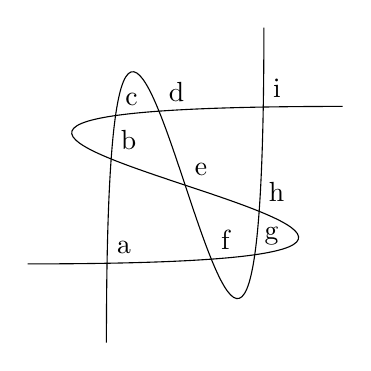
\begin{tikzpicture}
		\clip (-2, -2) rectangle (2, 2);
		\draw[name path=curve 1] (-2,-1) .. controls (8,-1) and (-8,1) .. (2,1);
		\draw[name path=curve 2] (-1,-2) .. controls (-1,8) and (1, -8) .. (1,2);
		\fill [name intersections={of=curve 1 and curve 2, sort by=curve 2, by={
							[label=above right:a],[label=above right:...], [label=above right:i]}}];
	\end{tikzpicture}
\end{texlst}

\section{相对坐标}
\texinline{+}和\texinline{++}是两个相对坐标操作符,区别在于\texinline{+}不改变当前的基点,而\texinline{++}操作后会将自身变为当前的基点。

旋转相对操作符\texinline{turn}
\begin{texlst}
	\begin{tikzpicture}
		\draw (0,0) -- (1,1) -- ([turn]-45:1cm) -- ([turn]-30:1cm);
	\end{tikzpicture}
\end{texlst}

\begin{texlst}
	\begin{tikzpicture}[delta angle=30, radius=1cm]
		\draw (0,0) arc [start angle=0] -- ([turn]0:1cm)
		arc [start angle=30] -- ([turn]0:1cm)
		arc [start angle=60] -- ([turn]30:1cm);
	\end{tikzpicture}
\end{texlst}

\texinline{turn}操作符还能接着\texinline{bend left/right}的角度继续变化。
\begin{texlst}
	\tikz \draw (0,0) to [bend left] (2,1) -- ([turn]0:1cm);
\end{texlst}
还可以接着\texinline{plots}后面。
\begin{texlst}
	\tikz \draw plot coordinates {(0,0) (1,1) (2,0) (3,0)} -- ([turn]30:1cm);
\end{texlst}

如果\texinline{turn}后面接的不是极坐标,比如\texinline{([turn]1,1)},这个效果相当于一个长度为$\sqrt2$偏角为$45^\circ$。
